\documentclass[10pt]{beamer}
\usepackage[utf8]{inputenc}
\usepackage[T1]{fontenc} 
\usepackage[croatian]{babel}
\usepackage{fix-cm}
\usetheme[progressbar=frametitle]{metropolis}
\usepackage{appendixnumberbeamer}
\usepackage{booktabs}
\usepackage{pgfplots}
\usepgfplotslibrary{dateplot}
\usepackage{xspace}
\graphicspath{ {slike/} }
\newcommand{\themename}{\textbf{\textsc{metropolis}}\xspace}
\usepackage{times}

\title{Git submoduli}
\subtitle{mogućnost korištenja repozitorija unutar repozitorija}
\date{}
\author{Dario Barać, Anđelo Ferenčić}

\begin{document}
\nocite{*}
\maketitle

%\begin{frame}{Table of contents}
% \setbeamertemplate{section in toc}[sections numbered]
%  \tableofcontents[hideallsubsections]
%\end{frame}


\begin{frame}{Uvod u git submodule}
\begin{itemize}
	\item Ako razvijamo projekt unutar kojeg se nalazi drugi projekt (npr. Bootstrap library unutar repozitorija web sjedišta) može doći do problema sa praćenjem njihovih verzija.
	\item Git taj problem riješava sa submodulima koji nam omogućuju njihovo neovisno verzioniranje.
\end{itemize}	
\end{frame}

\begin{frame}[fragile]{Početak rada sa submodulima}
 	U repozitoriju našeg web sjedišta ćemo inicijalizirati git submodul za Bootstrap library koristeći naredbu: \begin{semiverbatim}$submodule add \end{semiverbatim}
 	Submodul će biti spremljen u poddirektorij projekta i imat će isti naziv kao originalni repozitorij kojeg uključujemo.

	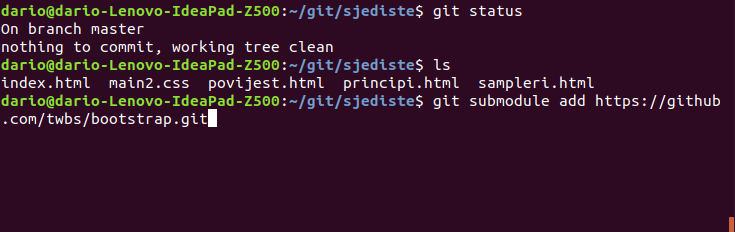
\includegraphics[scale=0.35]{submoduli_pocetak}
\end{frame}

\begin{frame}[fragile]{Početak rada sa submodulima}
	Naredba \begin{semiverbatim}$git status \end{semiverbatim} nam javlja daje stvorena .submodule datoteka koja sadrži imena i url adrese svih submodula. 

	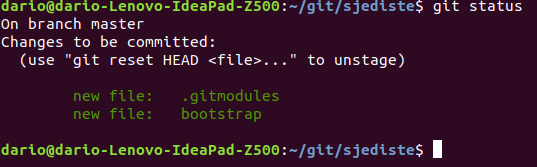
\includegraphics[scale=0.45]{submoduli_status}

	Možemo primjetiti i da git ne prati \emph{bootstrap}-ove datoteke jer zna da je to podrepozitorij.
\end{frame}

\begin{frame}{Početak rada sa submodulima}
	I kada napravimo \emph{commit} git prati podrepozitorije kao samo jednu datoteku.

	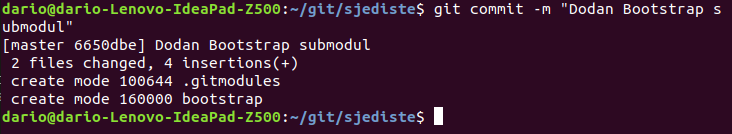
\includegraphics[scale=0.42]{sub_commit}

\end{frame}

\begin{frame}[fragile]{Kloniranje submodulima}
	Kada kloniramo repozitorij dobijemo dobijemo i prazan direktorij njegovih submodula. \\
	Sljedeće naredbe dohvaćaju sve datoteke koje su potrebne za rad podrepozitorija:
	\begin{semiverbatim}$git submodule init \end{semiverbatim}
	\begin{semiverbatim}$git submodule update \end{semiverbatim}
\end{frame}

\begin{frame}[fragile]{Kloniranje submodulima}
	Brža alternativa za to je da kod kloniranja dodamo i:
	\begin{semiverbatim} --recurse-submodules\end{semiverbatim}

	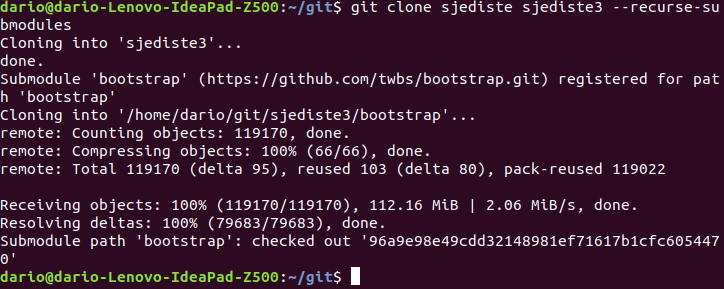
\includegraphics[scale=0.42]{sub_recurse}
\end{frame}

\begin{frame}[fragile]{Rad na projektima sa submodulima}
	Sadržaj podrepozitorija u našem projektu možemo ažurirati tako da unutar njihovih direktorija napišemo ove naredbe:
	\begin{semiverbatim}$git fetch\end{semiverbatim}
	\begin{semiverbatim}$git merge\end{semiverbatim}
	Ako imamo više podrepozitorija u projektu, ažuriranje nam može oduzeti dosta vremena.
\end{frame}

\begin{frame}[fragile]{Rad na projektima sa submodulima}
	To se rješava u glavnom direktoriju projekta sljedećom naredbom:
	\begin{semiverbatim}$git submodule update ---remote\end{semiverbatim}
	Time smo ažurirali sve submodule u našem projektu.

	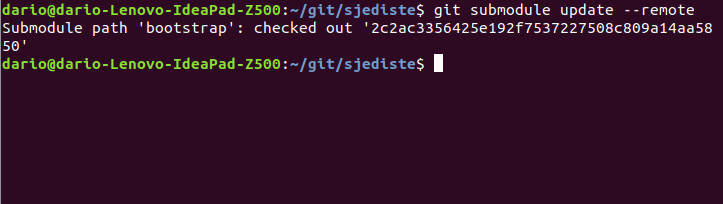
\includegraphics[scale=0.4]{sub_update}
\end{frame}

\begin{frame}[fragile]{Rad na projektima sa submodulima}
	\begin{semiverbatim}$git status\end{semiverbatim}
	U glavnom direktoriju javlja da imamo nove \emph{commitove} u podrepozitorijima.

	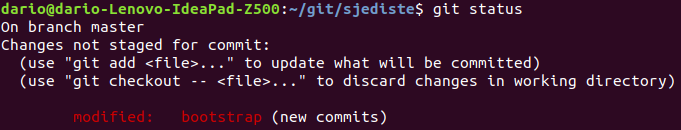
\includegraphics[scale=0.4]{sub_status2}

	\begin{semiverbatim}$git diff ---submodule\end{semiverbatim}
	Pokazuje koji su to \emph{commitovi}:

	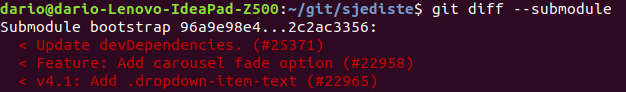
\includegraphics[scale=0.4]{sub_diff2}
\end{frame}

\begin{frame}[fragile]{Literatura}
	\bibliographystyle{ieeetr}
  	\bibliography{Pro_Git}
\end{frame}
\end{document}